v\documentclass{article}
\usepackage{algorithm}
\usepackage{algpseudocode}
\usepackage{svg}
\usepackage{color}
\usepackage{soul}
\usepackage{xcolor}
\usepackage{amsthm}
\usepackage{float}
\usepackage{sectsty}
\usepackage{amsbsy}
\usepackage{amsthm}
\usepackage{amsmath}
\usepackage{amsfonts}
\usepackage{graphicx}
\usepackage{multirow}
\usepackage{diagbox}
\usepackage{bm}
\usepackage{hhline}
\usepackage{graphicx}
\usepackage{helvet}
\usepackage{enumerate}
\usepackage{amsmath}
\usepackage{amsfonts}
\usepackage{graphicx}
\usepackage{multirow}
\usepackage{subfig}
\usepackage{comment}
\usepackage{mathtools}
\bibliographystyle{plain}

\newtheorem{Algorithm}{Algorithm}[section]
\newtheorem{Definition}{Definition}[section]
\newtheorem{Example}{Example}[section]
\newtheorem{Proposition}{Proposition}[section]
\newtheorem{Lemma}{Lemma}[section]
\newtheorem{Theorem}{Theorem}[section]
\newtheorem{Corollary}{Corollary}[section]
\newtheorem{Proof}{Proof}

\newcommand{\B}{{\mathbb{B}}}
\newcommand{\Z}{{\mathbb{Z}}}
\newcommand{\R}{{\mathbb{R}}}
\newcommand{\Q}{{\mathbb{Q}}}
\newcommand{\N}{{\mathbb{N}}}
\newcommand{\C}{{\mathbb{C}}}
\newcommand{\Zn}{{\mathbb{Z}}_{n}}
\newcommand{\Zp}{{\mathbb{Z}}_{p}}
\newcommand{\F}{{\mathbb{F}}}
\newcommand{\Fbar}{{\overline{\mathbb{F}}}}
\newcommand{\Fq}{{\mathbb{F}}_{q}}
\newcommand{\Jc}{J_c}
\newcommand{\Jz}{J_0}
\newcommand{\Jb}{J_b}
\newcommand{\Jt}{J_2}
\newcommand{\al}{\alpha}
\newcommand{\Joz}{J_1 + J_0}
\newcommand{\Jtz}{J_2 + J_0}
\newcommand{\Fqbar}{{\overline{{\mathbb{F}}_q}}}
\newcommand{\Fkk}{{\mathbb{F}}_{2^k}}
\newcommand{\Zkk}{{\mathbb{Z}}_{2^k}}
\newcommand{\Fkkx}[1][x]{\ensuremath{\mathbb{F}}_{2^k}[#1]\xspace}
\newcommand{\Grobner}{Gr\"{o}bner\xspace}
\newcommand{\bi}{\begin{itemize}}
\newcommand{\ei}{\end{itemize}}

\newcommand{\idealj}{{J = \langle f_1,f_2 \dots, f_s\rangle}}
\newcommand{\idealg}{{J = \langle g_1, \dots, g_t\rangle}}
\newcommand{\vfqj}{{V_{\Fq}(J)}}
\newcommand{\vfqjo}{{V_{\Fq}(J_0)}}
\newcommand{\vfbqj}{{V_{\overline{\Fq}}(J)}}
\newcommand{\vfbqjo}{{V_{\overline{\Fq}}(J_0)}}
\newcommand{\vfbqjjo}{{V_{\overline{\Fq}}(J+J_0)}}
\newcommand{\vfkkj}{{V_{\Fkk}(J)}}
% \newcommand{\v}{\vee}
\newcommand{\acf}{\bar{F}_q}
\newcommand{\Vacf}{V_{\bar{F}_q}}

\sectionfont{\large}

\title{The Unknown Component Problem}
\author{Vikas Rao\\
Department of  Electrical and Computer Eng.\\
University of Utah\\Vikas.k.rao@utah.edu }
\begin{document}

\maketitle
\section{Preliminaries}
Given a specification polynomial $f \in \Fq[x_1..x_n]=\R$ where $q=2^k$, and a circuit $C$ with $S$ gates. Write the gates as polynomials in $\R$ as $F=\{f_1,..,f_i,..,f_s\}: J=\langle f_1,..,f_i,..,f_s\rangle$. Let us consider $f_i$ to be the unknown component and of the special form $y_i+P(u_i)$, where $y_i$ is the leading term of the polynomial representing the unknown gate and $P$ as the function implementing the tail in terms of variables $u_i$, with $y_i\textgreater u_i$ as our variable order.

Let's assume that the circuit $C$ correctly implements $f$. Then $f\in I(\vfqj)=J+J_0: (J_0=\langle x_i^q-x_i\rangle)$, let's also assume $J\subset J_0$.

\begin{equation}\label{eq1}
\begin{split}
    f \in J \implies & f = h_1f_1+h_2f_2...+h_if_i+...+h_sf_s: \text{where } h_i\in\R\\
    & h_if_i = f + h_1f_1+h_2f_2...+h_{i-1}f_{i-1}+h_{i+1}f_{i+1}+...+h_sf_s\\
    & h_if_i \in \langle f,f_1,f_2...f_{i-1},f_{i+1}...f_s\rangle\\
\end{split}
\end{equation}

Let $J'$ represent this ideal $\langle f,f_1,f_2...f_{i-1},f_{i+1}...f_s\rangle$. Given the setup, can we project the variety of $J'$ on $y_i$ and $u_i$ coordinates and recover $f_i$?

\begin{align*}
    \text{Is } h_if_i \in J' \cap \fq[y_i,u_i]
\end{align*}
 
 \section{Debug Example}
 Consider the circuit given in fig.~\ref{tianka_ckt_c} with specification given as $f:z+a*c+a+b*c+b+c$ and variables from ring $\R=\F_2[z,z_1,z_2,d_0,e_2,e_1,e_0,a,b,c]$. Let us assume $f_4$ to be the unknown gate in the design.
 
 Polynomials for the given circuit are given as:
 \begin{equation}
 \begin{split}
 f_1 = e_0 + a + b; &\quad f_5 = z1 + e_0*d_0 + e_0 + d_0; \\
 f_2 = e_1 + b*c + b + c; &\quad f_6 = z_2 + d_0 + e_2; \\
 f_3 = e_2 + c + 1; &\quad f_7 = z + z_1*z_2; \\
 f_4 = d_0 + P(e_1,c);  
 \end{split}
 \end{equation}
 We shall add the vanishing polynomials of primary inputs, outputs, and intermediate variables and call this $ideal$ $J_0$. Here '$\al$' is the root of primitive polynomial used to build the field. 
\begin{align*}
 f_{8}:a^2 + a; &\quad f_{12}:e_1^2 + e_1; &\quad f_{16}:z_2^2 + z_2;\\
 f_{9}:b^2 + b; &\quad f_{13}:e_2^2 + e_2; &\quad f_{17}:z^2 + z;\\
 f_{10}:c^2 + c; &\quad f_{14}:d_0^2 + d_0; \\
 f_{11}:e_0^2 + e_0; &\quad f_{15}:z_1^2 + z_1; 
\end{align*}
 \begin{figure}[ht]
	\begin{center}
	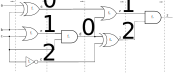
\includegraphics[scale = 0.80]{tianka_ckt_c}
	\end{center}
	\vspace{-4ex}
	\caption{circuit with redundancy}
	\label{tianka_ckt_c}
	\vspace{-2ex}
\end{figure}

From equation(\ref{eq1}):
\begin{gather}
\begin{split}
f \in \langle f_1,f_2...f_6,f_7\rangle: \text{ where } f_4 \text{ is unknown}\\
h_4f_4 \in \langle f,f_1,f_2,f_3,f_5,f_6,f_7\rangle\\
h_4f_4 = f+h_1f_1+h_2f_2+h_3f_3+h_5f_5+h_6f_6+h_7f_7
\end{split}
\end{gather}

Since we know that the unknown component lies between cuts $cut_0$ and $cut_1$, and given our RTTO$\textgreater$, we can compute $h_7,h_6,h_5 \text{, and} h_4$ with polynomial reduction as shown below.
We will be using the notations: '[]' to represent quotient-$h_i$'s, '()' to represent divisor-$f_i$'s, and '\{\}' to represent the partial remainder of every reduction step-$fp_i$'s.

Reduction order: $f_7\rightarrow f_6\rightarrow f_5\rightarrow f_4$

Variable order:$\{z,z_2,z_1,d_0,e_2,e_1,e_0,a,b,c\}$

\begin{gather*}
\begin{split}
f&\quad\xrightarrow[]{f_7}[1](z+z_2*z_1)+\{z_2*z_1+a*c+a+b*c+b+c\}\rightarrow fp_1\\
fp_1&\quad\xrightarrow[]{f_6}[z_1](z_2+d_0+e_2)+\{z_1*d_0+z_1*e_2+a*c+a+b*c+b+c\}\rightarrow fp_2\\
fp_2&\quad\xrightarrow[]{f_5}[d_0+e_2](z_1+d_0*e_0+d_0+e_0)+\{d_0*e_0*e_2+d_0*e_2+d_0+e_0*e_2+ac+a+bc+b+c\}\rightarrow fp_3\\
fp_3&\quad\xrightarrow[]{f_4}[e_0*e_2+e_2+1](d_0+P(e_1,c))+ \{fp_4\}
\end{split}
\end{gather*}

Equation (3) can now be re-written as:
\begin{gather*}
\begin{split}
h_4f_4+h_1f_1+h_2f_2+h_3f_3 = f+h_5f_5+h_6f_6+h_7f_7;\\
h_4(d_0+P(e_1,c))+h_1f_1+h_2f_2+h_3f_3 = f+h_5f_5+h_6f_6+h_7f_7;\\
h_4*d_0+h_4*P(e_1,c)+h_1f_1+h_2f_2+h_3f_3 = f+h_5f_5+h_6f_6+h_7f_7;\\
h_4*P(e_1,c)+h_1f_1+h_2f_2+h_3f_3 = h_4*d_0+f+h_5f_5+h_6f_6+h_7f_7;\\
h_4*P(e_1,c)+h_1f_1+h_2f_2+h_3f_3 = e_0*e_2+a*c+a+b*c+b+c;\\
h_4*P(e_1,c)+h_1f_1+h_2f_2+h_3f_3 = e_0*e_2+a*c+a+b*c+b+c;
\end{split}
\end{gather*}

Since, we know $h_4,f_1,f_2,f_3$, this can be formulated as ideal membership testing:
\begin{align}
e_0*e_2+a*c+a+b*c+b+c \in \langle h_4,f_1,f_2,f_3\rangle
\end{align}

Term re-writing(yet to figure it out in singular), we can arrive at:\\
\begin{lalign}\label{eq6}
e_0*e_2+a*c+a+b*c+b+c = [c](e_0*e_2+e_2+1)+[e_0*c+e_0+c](e_2 + c + 1)+\\
[0](e_1 + b*c + b + c)+[c+1](e_0 + a + b);
\end{lalign}

Thus, $P(u_1)=P(e_1,c)=c$, which can implemented as a simple AND gate with $c$ as both inputs. 

Since any $P_i$ which satisfies $P_i-P_j\in(f_1,f_2,f_3):h_4$, where $i\neq j$, works for the circuit, the computed $P$ is not considered unique and can take any values. We need to come up with better heuristics to identify the exact form and variables in which we want the $P$ to be. 

\bibliographystyle{ieeetr}
\bibliography{vikas}

\end{document}
